\documentclass{modernsimplecv}
% try out different fonts: classic, fira, raleway, chivo
\usepackage[utf8]{inputenc}
\usepackage[margin=1cm, a4paper]{geometry}

% ------------------------------------------------------------------------------------
% you can try out different fonts here by commenting the following lines in and out
% -----------------------------------------------------------------------------------
% \usepackage[default]{raleway}
%\usepackage[sfdefault]{FiraSans} %% option 'sfdefault' activates Fira Sans as the default text font\renewcommand*\oldstylenums[1]{{\firaoldstyle #1}}\normalfont
%\usepackage[familydefault,light]{Chivo} 
% \usepackage[sfdefault,light,condensed]{roboto}
\usepackage[default]{cantarell}
%\usepackage[sfdefault]{AlegreyaSans}


\usepackage{beuron}
\usepackage{LobsterTwo}%if not suposed to be main font, load other main font after this

\usepackage{hyperref}



%------------------------------------------------------------------ Variablen

\newlength{\rightcolwidth}
\newlength{\leftcolwidth}
\setlength{\leftcolwidth}{0.48\textwidth}
\setlength{\rightcolwidth}{0.47\textwidth}

%------------------------------------------------------------------
\title{modern-simple-CV}
\author{\LaTeX{} Ninja}
\date{August 2019}

\pagestyle{empty}
\begin{document}


\thispagestyle{empty}
%-------------------------------------------------------------



\tikz[remember picture,overlay] {%
\node[rectangle, fill=white, anchor=north, minimum width=\paperwidth, minimum height=5cm](header) at (current page.north){};%
}

\begin{minipage}[t]{0.21\textwidth}
\vspace{0pt} % Trick for alignment
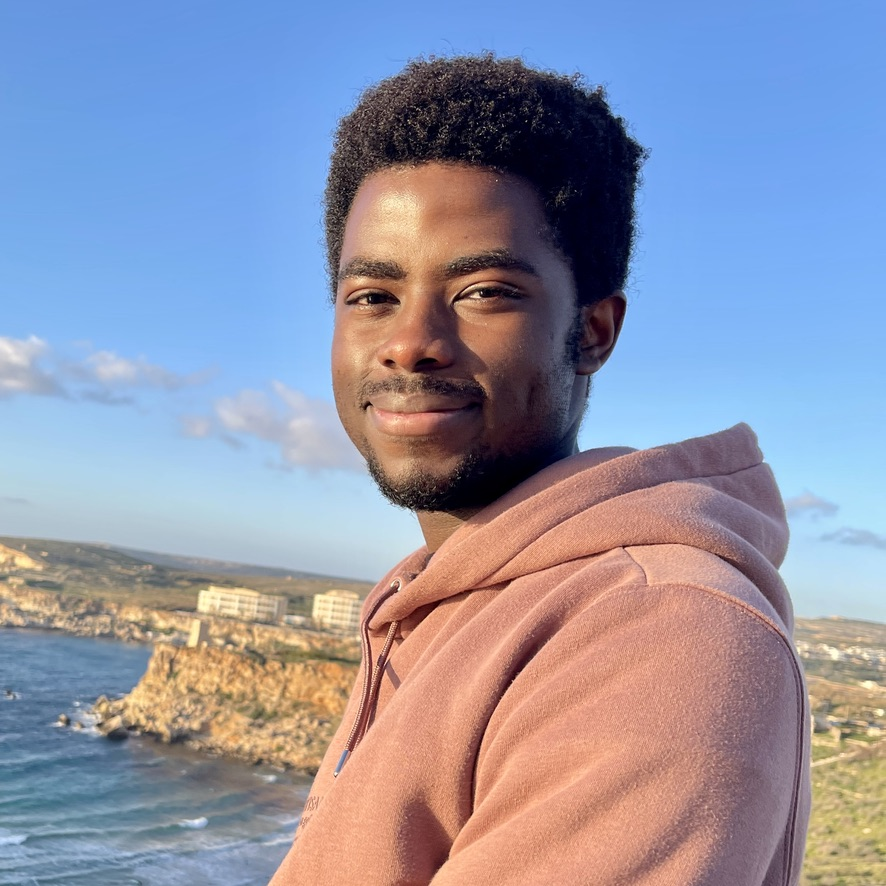
\includegraphics[width=\textwidth]{paul.jpeg}\hspace{1em}
\end{minipage}
\hfill
\begin{minipage}[t]{0.77\textwidth}
\vspace{0pt} % Trick for alignment
\begin{shaded*}

\begin{minipage}[t]{0.4\textwidth}
\vspace{0pt} % Trick for alignment
% here the fancy font can be taken out by removing \LobsterTwo
{\par\centering\huge\LobsterTwo{Paul Ashioya}} \\[0.3cm]
\faGlobe~ Nationality: Kenyan\\
\faBirthdayCake~ 13 June, 2001 \\
\faMapMarker~ Antwerpen, Belgium\\

{\small
\faCommentsO~ \underline{Languages:} \\ 
\emph{English}: Native \\ 
\emph{Kiswahilli}: Native \\ 
\emph{German}: B1 \\ 
\emph{Dutch}: A2\\
\emph{French}: A1\\}
\end{minipage}\hfill
\begin{minipage}[t]{0.55\textwidth}
\vspace{0pt} % Trick for alignment
\faPhone~ +32 456036814 \\
\faAt~ {john.ashioya@gmail.com} \\

%\aiAcademiaSquare 
\faFont~ \protect\url{pashioya.com (under-renovation)} \\
\faGithub~ \protect\url{https://github.com/pashioya} \\
\faGitlab~ \protect\url{https://gitlab.com/pashioya} \\
%\aiOrcid 
\end{minipage}
\hfill
\end{shaded*}
\end{minipage}\\[15pt]


%------------------------------------------------

\subsection*{}
\vspace{-3em}

\setlength{\columnsep}{1.5cm}
\columnratio{0.48}[0.47]
\begin{paracol}{2}
\hbadness5000
%\backgroundcolor{c[1]}[rgb]{1,1,0.8} % cream yellow for column-1 %\backgroundcolor{g}[rgb]{0.8,1,1} % \backgroundcolor{l}[rgb]{0,0,0.7} % dark blue for left margin

\paracolbackgroundoptions

% 0.9,0.9,0.9 -- 0.8,0.8,0.8


\footnotesize
{

\small
\section*{Resumé}

\begin{minipage}[t]{\leftcolwidth}
\begin{tabular}{r| p{0.6\textwidth} c}
    \cvevent{2022--2024}{CityBox Antwepen}{Host}{Antwerp-Belgium}{Although the hotel is mostly automated, I ensured all systems were running as expected while answering all calls and guests questions.}{citybox.png} \\
    \cvevent{2024--2024}{Tryve EU}{Internship}{Antwerpen}{I am responsible for the development of the companys new mobile app utilizing tryves existing infrastructure, to create a on-the-go location based task manager for on site workers}{tryve.png} \\
\end{tabular}

\vspace{4em}

\end{minipage}

\begin{minipage}[t]{\leftcolwidth}
\section*{Degrees}
\begin{tabular}{r p{0.6\textwidth} c}
    \cvdegree{2017 - 2018}{(Partial) Applied Computer Technology}{B.S.}{ United States International University - Africa}{}{usiu.png} \\
    \cvdegree{2018 - 2021}{International Baccalaureate}{I.B.}{Berlin International School}{}{ib.png} \\
    \cvdegree{2020 - 2021 }{(Partial) Computer Science}{B.S.}{International University of Applied Science - Berlin}{}{iubh.png} \\
    \cvdegree{2021 - 2024}{Applied Computer Science}{B.S.}{Karel de Grote - Antwerp}{}{kdg.png} 
\end{tabular}
\end{minipage}\hfill

\vspace{3em}

\begin{minipage}[t]{\leftcolwidth}

\end{minipage}\hfill


\vspace{2em}

\begin{minipage}[t]{\leftcolwidth}
\section*{Favourite Projects}
\begin{tabular}{r| p{0.6\textwidth} c}
    \cvevent{2023}{Youth Council Project}{Developer}{KdG}{The Youth Council Project is a web application that allows young people to express their ideas on how to improve their community}{disney.png} \\
    \cvevent{2023}{Tech-Topia Themepark}{Developer}{KdG}{I designed a comprehensive theme park management software, encompassing features like visitor ticketing, ride check-in systems, and weather-based forecasting for visitor traffic.  (Optional addition): To enhance the visitor experience, I also built a front-end project replicating a theme park's information system.}{medal.jpeg} \\
    \cvevent{2016--2017}{The Machine Learners}{Developer}{KdG}{This project tackles the Cartpole and Frozen Lake problems using both tabular and deep learning approaches. The Cartpole environment, where an agent learns to balance a pole on a moving cart, is solved with a Deep Q-Network (DQN) implemented in TensorFlow, achieving success in under 1000 episodes (training iterations) on CPU alone.}{medal.jpeg} \\
    \cvevent{2018--2021}{TuhBehHuh}{Developer}{KdG}{This project helps you breathe easy! It analyzes air quality (pollution, pollen), traffic, weather, and dust, letting you know if it's safe to go outside. Set custom notifications for anomalies, forecasts, and historical data, and even monitor other locations. It fosters community by notifying you of air quality anomalies and inviting you to share insights.}{disney.png}
\end{tabular}

\vspace{4em}
\end{minipage}
}
%-----------------------------------------------------------
\switchcolumn

\section{Introduction} 
{\small
Highly motivated international student from Kenya, graduating with a Bachelor of Science degree in Computer Science with a specialization in Artificial Intelligence. Possessing a strong foundation in programming and a passion for full-stack development, I am eager to leverage my skills and knowledge to contribute to a dynamic team environment.
}
\bigskip


\subsection*{Backend}

\begin{skillsection}{\rightcolwidth}
    \cvitem{\faStar\faStar\faStar\faStar\faStarO}{Java}
    \cvitem{\faStar\faStar\faStar\faStar\faStarO}{NodeJs}
    \cvitem{\faStar\faStar\faStar\faStarO\faStarO}{Rust}
\end{skillsection}

\subsection*{Frontend}

\begin{skillsection}{\rightcolwidth}
    \cvitem{\faStar\faStar\faStar\faStar\faStarO}{React + React Native}
    \cvitem{\faStar\faStar\faStar\faStarO\faStarO}{Solid}
    \cvitem{\faStar\faStar\faStarO\faStarO\faStarO}{Leptos}
\end{skillsection}

\subsection*{DevOps}

\begin{skillsection}{\rightcolwidth}
    \cvitem{\faStar\faStar\faStar\faStar\faStarO}{Azure}
    \cvitem{\faStar\faStar\faStar\faStar\faStarO}{G-Cloud}
    \cvitem{\faStar\faStar\faStarO\faStarO\faStarO}{AWS}
    \cvitem{\faStar\faStar\faStarO\faStarO\faStarO}{Terraform}
\end{skillsection}

\subsection*{Data \& AI}


\begin{skillsection}{\rightcolwidth}
    \cvitem{\faStar\faStar\faStar\faStarHalfO\faStarO}{Python, Machine Learning, Forecasting...}
    \cvitem{\faStar\faStar\faStarO\faStarO\faStarO}{Rust}
\end{skillsection}

\bigskip



\vspace{4em}


\begin{minipage}[t]{\rightcolwidth}
\section*{Publications (Hint: Click on Article)}
\begin{tabular}{>{\footnotesize\bfseries}r >{\footnotesize}p{0.7\textwidth}}
2024 & \emph{\href{https://medium.com/@john.ashioya/third-life-simulating-reality-14d7663896dd}{Third Life: Simulating Reality}}, Karel de Grote. \\
\end{tabular}
\bigskip
\end{minipage}
\end{paracol}

\vfill{} % Whitespace before final footer
%----------------------------------------------------------------------------------------
%	FINAL FOOTER
%----------------------------------------------------------------------------------------
\setlength{\parindent}{0pt}
\begin{minipage}[t]{\textwidth}
\begin{center}\fontfamily{\sfdefault}\selectfont \color{black!70}
{\small Paul Ashioya \icon{\faMapMarker}{black}{} Antwerpen \icon{\faPhone}{black}{} +32 456036814 
\icon{\faAt}{black}{} {john.ashioya@gmail.com}
}
\end{center} 
\begin{center}  \color{gray}
    {
        Written in LaTeX. Source code available on \protect\url{https://github.com/pashioya/pauls-cv}
    }
\end{center}
\end{minipage}

\end{document}
